%\subsection{Explicit formula of NTK}\label{subsec:A_ExplicitNTK}
%
%Let us first recollect some definition and properties of the arc-cosine kernels introduced in \citet{cho2009_KernelMethods}.
%\begin{definition}[Arc-cosine kernels]
%  \label{def:ACK}
%  Let $\sigma(x) = \max(x,0)$ be the ReLU function.
%  The arc-cosine kernel of order $n$ is defined by
%  \begin{align}
%    \label{eq:D_AnDef}
%    A_n(\x,\y) &\coloneqq 2 \E_{\bm{w} \sim N(0,I_n)} \left[
%      \sigma(\ang{\x,\bm{w}})^n \sigma(\ang{\y,\bm{w}})^n \right],
%  \end{align}
%  where we use the convention that $0^n = 0$ when $n=0$.
%  Furthermore, one can easily find that there is a function $\kappa_n$ defined on $[-1,1]$ such that
%  \begin{align}
%    A_n(\x,\y) = \norm{\x}^n \norm{\y}^n \kappa_n\left(\frac{\ang{\x,\y}}{\norm{\x}\norm{\y}}\right).
%  \end{align}
%\end{definition}
%
%%The following explicit formula of the arc-cosine kernel  $\kappa_{0}$ and $\kappa_{1}$ is borrowed from \citep{cho2009_KernelMethods}.
%\begin{proposition}
%  \label{prop:ACK01}
%  We have the following explicit expression of the arc-cosine kernels:
%  \begin{align}
%    \label{eq:A_Kappa0}
%    \kappa_0(u) &= \frac{1}{\pi}\left( \pi - \theta \right) = \frac{1}{\pi}\left( \pi - \arccos u \right),\\
%    \label{eq:A_Kappa1}
%    \kappa_1(u) &= \frac{1}{\pi}\left[ \sin \theta + (\pi - \theta) \cos \theta \right] = \frac{1}{\pi}\left[ \sqrt {1-u^2} + u (\pi - \arccos u)  \right],
%  \end{align}
%  where $\theta = \theta(u) = \arccos u$ is the angle between two vectors.
%\end{proposition}
%
%The connection between arc-cosine kernel and NTK defined through the recursion formula (10) in the main text is given by the following proposition:
%\begin{proposition}
%  \label{prop:D_ACK_NTK}
%  Let $B = \mqty(a^2 & \rho ab \\ \rho ab & b^2)$ for $\rho \in [-1,1]$.
%  We have
%  \begin{align}
%    2\E_{(u,v) \sim N(0,B)}\left[ \sigma'(u) \sigma'(v) \right] = \kappa_0(\rho),
%    \quad 2\E_{(u,v) \sim N(0,B)}\left[ \sigma(u) \sigma(v) \right] = ab \kappa_1(\rho).
%  \end{align}
%\end{proposition}
%\begin{proof}
%  Letting $u = \ang{\x,\bm{w}}$ and $v = \ang{\y,\bm{w}}$ in the definition \cref{eq:D_AnDef} of $A_n(\x,\y)$ and noticing that
%  $(u,v) \sim N(0, \bm{\Lambda})$ for $\bm{\Lambda} = \mqty(\norm{\x}^2 & \ang{\x,\y} \\ \ang{\x,\y} & \norm{\x}^2)$,
%  we get
%  \begin{align*}
%    2 \E_{(u,v) \sim N(0,\bm{\Lambda})}\left[\sigma(u)^n \sigma(v)^n\right] =
%    A_n(\x,\y) = \norm{\x}^n \norm{\y}^n \kappa_n\left(\frac{\ang{\x,\y}}{\norm{\x}\norm{\y}}\right).
%  \end{align*}
%  The proof is then finished by setting $a = \norm{\x},~ b = \norm{\y},~\rho = \frac{\ang{\x,\y}}{\norm{\x}\norm{\y}}$
%  and noticing that $\sigma^0(\x) = \sigma'(\x) = \bm{1}\{\x > 0\}$.
%\end{proof}
%
%Using \cref{prop:D_ACK_NTK}, we can rewrite the recursion formula (9) and (10) in the main text as
%\begin{align}
%  \label{eq:NTK_DefRecur1}
%  \begin{aligned}
%    \Sigma_0(\x,\y) &= N_0(\x,\y) = \ang{\x,\y} + 1, \\
%    \Sigma_{l}(\x,\y) &=
%    \sqrt {\Sigma_{l-1}(\x,\x) \Sigma_{l-1}(\y,\y)}~  \kappa_1\left( \frac{\Sigma_{l-1}(\x,\y)}{\sqrt {\Sigma_{l-1}(\x,\x) \Sigma_{l-1}(\y,\y)}} \right), \\
%    N_{l}(\x,\y) &= \Sigma_{l}(\x,\y) + N_{l-1}(\x,\y) \kappa_0\left( \frac{\Sigma_{l-1}(\x,\y)}{\sqrt {\Sigma_{l-1}(\x,\x) \Sigma_{l-1}(\y,\y)}} \right).
%  \end{aligned}
%\end{align}
%Now let us denote $\tilde{\x} = (\x,1),~\tilde{\y} = (\y,1)$.
%Since from \cref{prop:ACK01} we know that $\kappa_0(1) = \kappa_1(1) = 1$,
%letting $x=y$ in the recursion formula of $\Sigma_l$ leads to
%\begin{align*}
%  \Sigma_{l}(\x,\x) &= \Sigma_{l-1}(\x,\x) = \dots = \Sigma_{0}(\x,\x) = \norm{\tilde{\x}}^2.
%\end{align*}
%Plugging it back into the recursion formula, we get
%\begin{align*}
%  \frac{\Sigma_{l}(\x,\y)}{\norm{\tilde{\x}}\norm{\tilde{\y}}} =
%  \kappa_1\left( \frac{\Sigma_{l-1}(\x,\y)}{\norm{\tilde{\x}}\norm{\tilde{\y}}} \right)
%\end{align*}
%and thus $\Sigma_l(\x,\y) = \norm{\tilde{\x}}\norm{\tilde{\y}} \kappa^{(l)}_1(\bar{u})$,
%where we define $\bar{u} = \frac{\ang{\tilde{\x},\tilde{\y}}}{\norm{\tilde{\x}}\norm{\tilde{\y}}}$.
%Therefore, expanding the recursion formula of $N_l$, we get
%\begin{align}
%  \notag
%  N_l(\x,\y) &= \Sigma_l(\x,\y) + N_{l-1}(\x,\y) \kappa_0 (\kappa^{(l-1)}_1(\bar{u}))
%  = \sum_{r=0}^l \Sigma_{l-r}(\x,\y) \prod_{s=1}^r \kappa_0(\kappa^{(l-s)}_1(\bar{u})) \\
%  &= \norm{\tilde{\x}}\norm{\tilde{\y}} \sum_{r=0}^l \kappa^{(r)}_1(\bar{u}) \prod_{s=r}^{l-1} \kappa_0(\kappa^{(s)}_1(\bar{u})).
%\end{align}
%Finally, we conclude the result as (15) in the main text:
%\begin{align*}
%  \NTK(\x,\y) =
%  \norm{\tilde{\x}}\norm{\tilde{\y}} \sum_{r=0}^l \kappa^{(r)}_1(\bar{u}) \prod_{s=r}^{l-1} \kappa_0(\kappa^{(s)}_1(\bar{u})) + 1.
%\end{align*}
%
%%\begin{align}
%%  \Sigma_l(\x,\y) &= \norm{\tilde{\x}}\norm{\tilde{\y}} \kappa^{(l)}_1(\bar{u}), \\
%%  N_l(\x,\y) &= \norm{\tilde{\x}}\norm{\tilde{\y}} \sum_{r=0}^l \kappa^{(l-r)}_1(\bar{u}) \prod_{s=1}^r \kappa_0(\kappa^{(l-s)}_1(\bar{u}))
%%\end{align}
%

%\subsection{Spectral properties of $\NTK$}
%Let us introduce a map
%$\Phi:\mathbb R^{d} \rightarrow \bbS^{d}_{+}$ given by $\x\mapsto \frac{(\x,1)}{\|(\x,1)\|}$,
%where we denote $\mathbb{S}^{d}_{+}\coloneqq\{\x=(x_{1},\ldots,x_{d+1})\in \mathbb{S}^{d}\mid x_{d+1}>0\}$.
%It is easy to verify that for any bounded open set $\Omega \subset \mathbb R^{d}$,
%$\Phi$ is a diffeomorphism from $\Omega$ to $\Phi(\Omega)$ and the Jacobian $J\varphi$ satisfies $0 < c \leq \abs{J\Phi} \leq C < \infty$ for some constants $c$ and $C$.
%Recalling \cref{eq:NTK_Formula}, we have
%\begin{align}
%  \label{eq:NTK_Pullback}
%  \NTK(\x,\x') =
%  \norm{\tilde{\x}}\norm{\tilde{\x}'} \sum_{r=0}^l \kappa^{(r)}_1(\bar{u}) \prod_{s=r}^{l-1} \kappa_0(\kappa^{(s)}_1(\bar{u})) + 1
%  =
%  \norm{\tilde{\x}}\norm{\tilde{\x}'} (\Phi^{*}\NTK_{0})(\x,\x') + 1,
%\end{align}
%where $\NTK_0$ is a kernel on $\bbS^d$ given in \cref{eq:NTK0_Def} and $\Phi^{*}\NTK_{0}$ is the pull-back kernel.
%where $\tilde{\x} = (\x,1)$, $\tilde{\y} = (\y,1)$, and $\bar{u} = \frac{\ang{\tilde{\x},\tilde{\y}}}{\norm{\tilde{\x}}\norm{\tilde{\y}}}$.

%Let us consider the kernel
%\begin{align}
%  \label{eq:NTK0_Def}
%  \NTK_0(\x,\y) =  \sum_{r=0}^l \kappa^{(r)}_1(u)  \prod_{s=r}^{l-1} \kappa_0(\kappa^{(s)}_1(u)),\quad
%  u = \ang{\x,\y},\quad \x,\y\in \bbS^d,
%\end{align}
%defined on $\bbS^{d}$.
%The following result is given in \citet{bietti2020_DeepEquals}.
%
%\begin{proposition}
%  \label{prop:NTK0_EDR}
%  For the homogeneous $\NTK_{0}$ defined in \cref{eq:NTK0_Def},
%  the coefficients $\mu_n$ in the decomposition \cref{eq:C_Mercer} satisfy
%  \begin{align}
%    \mu_n \asymp n^{-(d+1)}.
%%    \lambda_i(\mathrm{NTK}_0;\bbS^d,\dd \sigma) \asymp i^{-\frac{d+1}{d}}.
%  \end{align}
%\end{proposition}

\subsection{Positive definiteness}
\label{subsec:D_PDNTK}

The following proposition is an elementary result on the power series expansion of the arc-cosine kernels.
\begin{proposition}
  \label{prop:D_ACK_PS}
  We have the following power series expansion for $\kappa_0$ and $\kappa_1$ in \cref{eq:Arccos_Formula}:
  \begin{align}
    \kappa_0(u) &= \frac{1}{2} + \frac{1}{\pi} \sum_{r=0}^\infty \frac{\left(\frac{1}{2}\right)_r}{(2r+1) r!} u^{2r+1},
    \quad
    \kappa_1(u) = \frac{1}{\pi} + \frac{1}{2}u + \frac{1}{\pi} \sum_{r = 1}^{\infty} \frac{\left(\frac{1}{2}\right)_{r-1}}{2(2r-1) r!} u^{2r},
  \end{align}
  where $(a)_p \coloneqq a(a+1)\dots(a+p-1)$ represents the rising factorial
  and both series converge absolutely for $u \in [-1,1]$.
%  \sqrt {1-\x^2} &= 1 - \sum_{r=1}^{\infty} \frac{\left(\frac{1}{2}\right)_{r-1}}{2 r!} \x^{2r} \\
\end{proposition}

\begin{lemma}
[Lemma B.1 in \citet{lai2023_GeneralizationAbility}]
  \label{lem:B_PDSphere}
  Let $f: [-1,1] \to \R$ be a continuous function with the expansion
  $f(u) = \sum^{\infty}_{n=0}a_n u^n, \quad u \in [-1,1]$
  and $k(x,y) = f(\ang{x,y})$ be the associated inner-product kernel on $\bbS^{d}$.
  If $a_{n}\geq 0$ for all $n \geq 0$ and there are infinitely many $a_n > 0$, then $k$ is
  positive definite on $\mathbb{S}^{d}_{+}$.
\end{lemma}


%Thus, we know that $\NTK$ is positive definite since $\norm{\tilde{\x}}\geq 1$ for $x \in \R^d$
%and $\NTK_0$ is positive definite on $\bbS_{+}^{d}$.

%\iffalse
%  We recall that the NTK is given by
%  \begin{align*}
%    \NTK(\x,\y) =
%    \norm{\tilde{\x}}\norm{\tilde{\y}} \sum_{r=0}^l \kappa^{(r)}_1(\bar{u}) \prod_{s=r}^{l-1} \kappa_0(\kappa^{(s)}_1(\bar{u})) + 1.
%  \end{align*}
%  where $\tilde{\x} = (\x,1)$, $\tilde{\y} = (\y,1)$, $\bar{u} = \frac{\ang{\tilde{\x},\tilde{\y}}}{\norm{\tilde{\x}}\norm{\tilde{\y}}}$.
%  Using (1),(3) in \cref{lem:B_PDSumProd} with $\rho(\x) = \norm{\tilde{\x}}\geq 1$ for $x \in \R^d$,
%  it suffices to prove that
%  \begin{align}
%    \label{eq:D_K1}
%    K_1 = \sum_{r=0}^l \kappa^{(r)}_1(\bar{u}) \prod_{s=r}^{l-1} \kappa_0(\kappa^{(s)}_1(\bar{u}))
%  \end{align}
%  is positive definite.
%
%  Consider the mapping $\varphi_1 : \R^d \to \R^d \times \{1\}$ given by $\x \mapsto \tilde{\x} = (\x,1)$,
%  $\varphi_2 : \R^d \times \{1\} \to \bbS^d_+$ given by $\tilde{\x}\mapsto \frac{\tilde{\x}}{\norm{\tilde{\x}}}$
%  and $\varphi = \varphi_2 \circ \varphi_1 : \R^d \to \bbS^d_+$, where
%  $\bbS^d_+ = \{(x_{1},\ldots,x_{d+1})\in \mathbb{S}^{d}\mid x_{d+1}>0\}$
%  is the half sphere.
%  It is easy to verify that $\varphi$ is an injection and the pull-back kernel $\varphi^* K_1 = \NTK_0$ as
%  defined in \cref{eq:NTK0_Def}:
%  \begin{align*}
%    \NTK_0(\x,\y) =  \sum_{r=0}^l \kappa^{(r)}_1(u)  \prod_{s=r}^{l-1} \kappa_0(\kappa^{(s)}_1(u)),\quad
%    u = \ang{\x,\y},\quad \x,\y\in \bbS^d_+.
%  \end{align*}
%
%  Finally, the positive definiteness of $\NTK_0$ on $\bbS^d_+$ follows from (3) in \cref{lem:B_PDSphere} using
%  the power series expansion of $\kappa_0$ and $\kappa_1$ given in \cref{prop:D_ACK_PS}.
%\fi


\begin{proof}
[of \cref{prop:NTK_PD}]
  Following the proof of \cref{thm:NTK_EDR}, we introduce the transformation $\Phi$ and the homogeneous NTK $\NTK_0$.
  Plugging \cref{prop:D_ACK_PS} into \cref{eq:NTK0_Def}, by \cref{lem:B_PDSphere} we can show that $\NTK_0$ is strictly positive definite on
  $\bbS_{+}^{d} = \Phi(\R^d)$.
  Consequently, the positive definiteness of $\NTK$ follows from the fact that $\Phi$ is bijective and $\norm{\tilde{x}} \geq 1$.
\end{proof}

%\subsubsection{Eigenvalue decay rate of $\NTK$}
%\label{subsubsec:D_PfEDR}
%In the following we directly prove the eigenvalue decay rate of $\NTK$, which will include the proof of \cref{lem:NTK_pf_reduce}.
%
%First, \cref{thm:EDRS} and \cref{prop:NTK0_EDR} yield
%\begin{align*}
%  \lambda_i(\NTK_0;S,\dd \sigma) \asymp \lambda_i(\NTK_0;\bbS^d,\dd \sigma) \asymp i^{-\frac{d+1}{d}},
%\end{align*}
%where $S = \Phi(\caX)$ is an open set.
%Then, using \cref{lem:B_DiffeoKernel}, \cref{lem:B_ScaledKernel} together with \cref{prop:Eigen_ChangeOfMeasure} and $\norm{\tilde{x}} \geq 1$, we get
%\begin{align*}
%%  \lambda_i(\NTK;\caX,\dd \mu)
%  \lambda_i(\NTK_{0};S, \dd \sigma)  \asymp \lambda_i(\Phi^{*}\NTK_{0};\caX, \dd \x)
%  \asymp  \lambda_i(\norm{\tilde{\x}}\norm{\tilde{\x}'}\Phi^{*}\NTK_{0};\caX,\dd \mu).
%\end{align*}
%Finally, by the expression \cref{eq:NTK_Pullback} and the fact that an extra constant $1$ will not affect the eigenvalue decay $i^{-\frac{d+1}{d}}$,
%we conclude
%\begin{align*}
%  \lambda_i(\NTK;\caX,\dd \mu)
%  \asymp \lambda_i(\norm{\tilde{\x}}\norm{\tilde{\x}'}\Phi^{*}\NTK_{0};\caX,\dd \mu)
%  \asymp i^{-\frac{d+1}{d}}.
%\end{align*}
%%  where $S = \Phi(\caX) \subset \bbS^d_+$ is an open set.
%
%%  Then, \cref{thm:EDRS} and \cref{prop:NTK0_EDR} yield that
%%  \begin{align*}
%%      \lambda_i(\NTK_{0};S, \dd \sigma) \asymp \lambda_i(\NTK_{0};\bbS^d, \dd \sigma) \asymp i^{-\frac{d+1}{d}}
%%  \end{align*}
%%
%%%  where $\Omega$ is the interior of $\caX$.
%%%  Let $K_1$ be the kernel defined in \cref{eq:D_K1}.
%%  Noticing $\NTK(\x,\y) = \norm{\tilde{\x}}\norm{\tilde{\y}} \Phi^{*}\NTK_0(\x,\y) + 1$,
%%  we have
%%  \begin{align*}
%%    \lambda_i(\NTK;\Omega,\dd \x) \asymp \lambda_i(\norm{\tilde{\x}}\norm{\tilde{\y}} \Phi^{*}\NTK_0;\Omega,\dd \x)
%%    \asymp \lambda_i(\Phi^{*}\NTK_0;\Omega,\dd \x),
%%  \end{align*}
%
%% Moreover, the pull-back kernel $\Phi^* K_1 = \NTK_0$ as defined in \cref{eq:NTK0_Def}.
%%Let $S = \Phi(\Omega)$ be the image of $\Phi$.
%%  Then, by \cref{lem:B_DiffeoKernel}, we obtain
%%  \begin{align*}
%%    \lambda_i(\Phi^{*}\NTK_0;\caX,\dd \x) = \lambda_i(\Phi^{*}\NTK_0;\Omega,\dd \x) \asymp \lambda_i(\NTK_0;\Phi(\Omega),\dd \sigma).
%%  \end{align*}
%%
%%  Finally, the assumed polynomial decay rate can be seen from applying \cref{thm:EDRS} and \cref{prop:NTK0_EDR},
%%  , and thus
%%  $\lambda_i(\norm{\tilde{\x}}\norm{\tilde{\y}} K_1;\Omega,\dd \x) \asymp i^{-\frac{d+1}{d}} $.
%%\end{proof}

%This subsection is devoted to prove \cref{thm:NTK_EDR}.

\subsection{Numerical experiments}


\begin{figure*}[t]
  \centering
  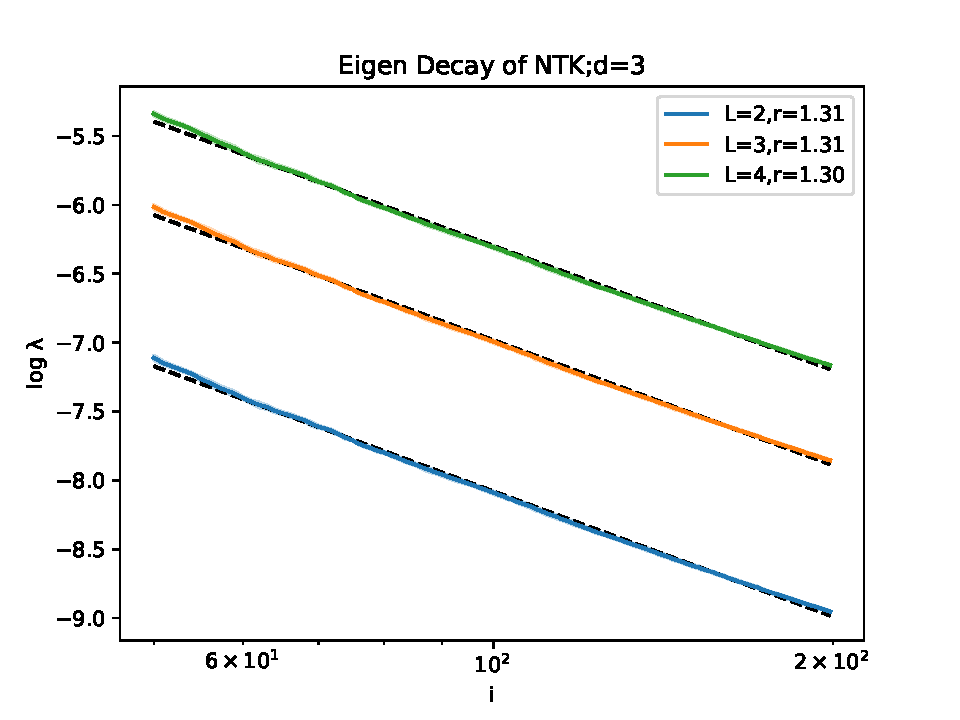
\includegraphics[width=0.49\textwidth]{fig/EigenNTKd3}
  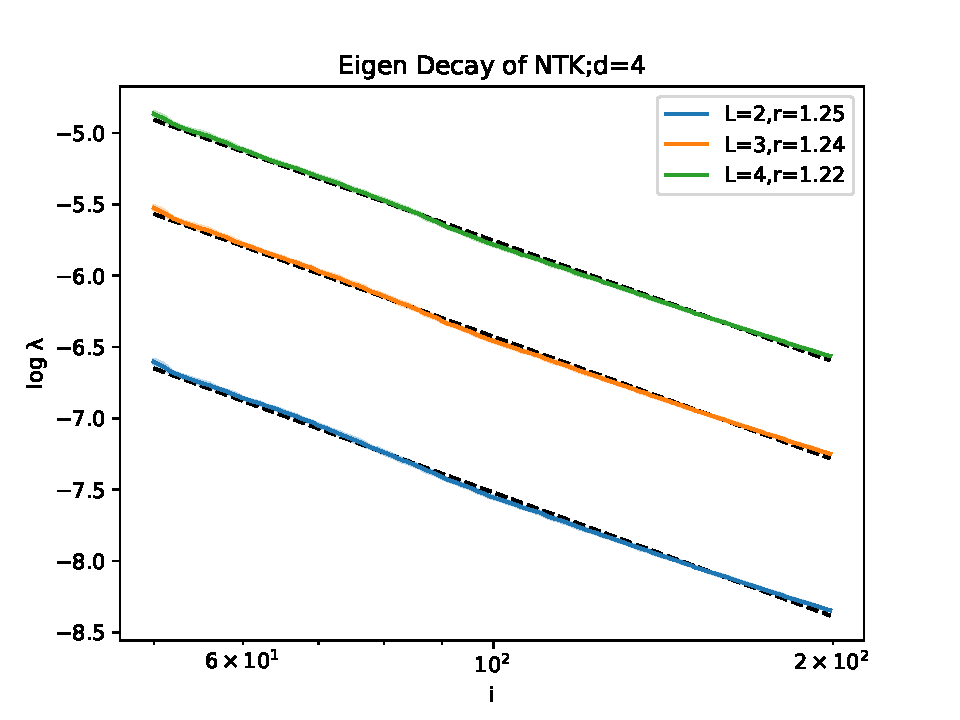
\includegraphics[width=0.49\textwidth]{fig/EigenNTKd4}
  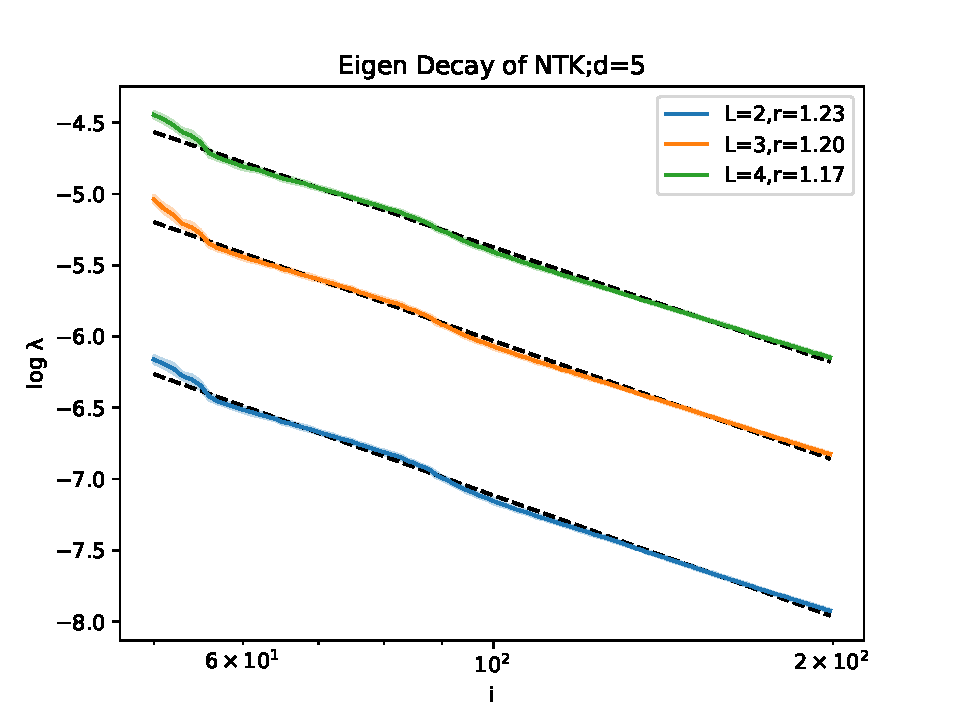
\includegraphics[width=0.49\textwidth]{fig/EigenNTKd5}
  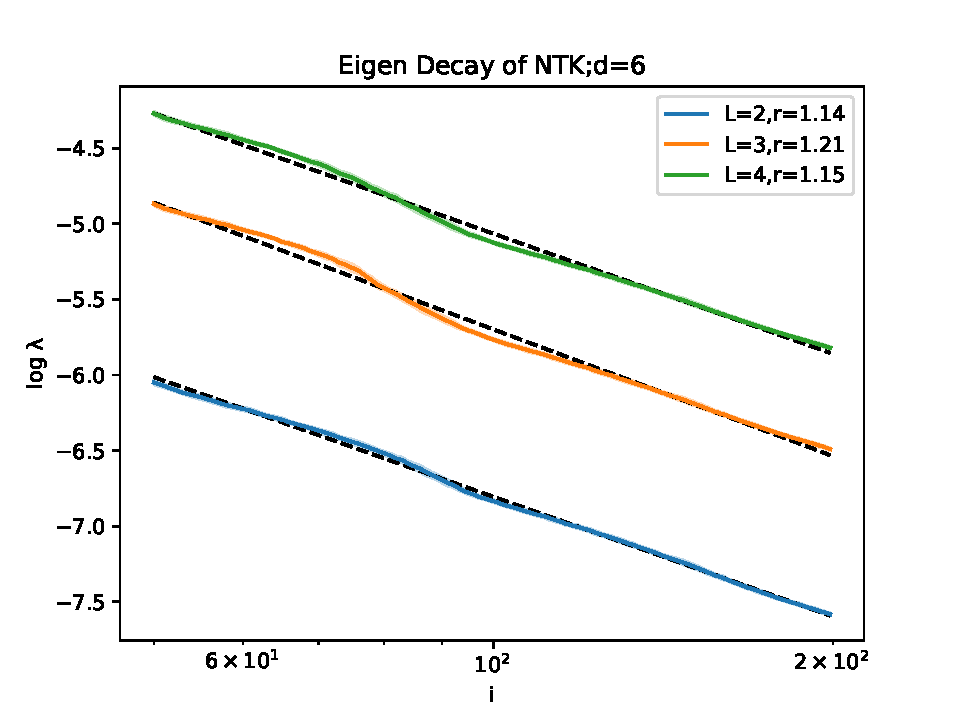
\includegraphics[width=0.49\textwidth]{fig/EigenNTKd6}
  \caption{Eigenvalue decay of NTK under uniform distribution on $[-1,1]^d$,
    where $i$ is selected in $[50,200]$ and $n = 1000$.
    The dashed black line represents the log least-square fit and the decay rates $r$ are reported.}
  \label{fig:EDR1}
\end{figure*}
\begin{table*}[t]
  \centering
  \begin{tabular}{c|ccc|ccc|ccc}
    & \multicolumn{3}{c|}{$d=3$} & \multicolumn{3}{c|}{$d=4$} & \multicolumn{3}{c}{$d=5$} \\
    \hline
    Distribution   & $L=2$ & $L=3$ & $L=4$ & $L=2$ & $L=3$ & $L=4$ & $L=2$ & $L=3$ & $L=4$ \\
    \hline
    $U(-1,1)$      & 1.31  & 1.31  & 1.30  & 1.25  & 1.24  & 1.22  & 1.23  & 1.20  & 1.17  \\
    $U(0,1)$       & 1.33  & 1.33  & 1.32  & 1.26  & 1.26  & 1.25  & 1.14  & 1.13  & 1.12  \\
    Triangular     & 1.34  & 1.33  & 1.32  & 1.21  & 1.23  & 1.22  & 1.22  & 1.16  & 1.13  \\
    Clipped normal & 1.28  & 1.30  & 1.28  & 1.26  & 1.24  & 1.21  & 1.11  & 1.09  & 1.06
  \end{tabular}
  \caption{Eigenvalue decay rates of NTK, where each entry of $\x$ is drawn independently from multiple distributions.
  Triangular: $p(\x) = 1+x$, $x \in [-1,0]$, $p(\x) = 1-x$, $x \in [0,1]$;
  Clipped normal: standard normal clipped into $(-10,10)$.}
  \label{tab:1}
\end{table*}


We provide some numerical experiments on the eigenvalue decay of the neural tangent kernel.
%Since we have the convergence \cref{thm:EigenvalueConvergence},
We approximate the eigenvalue $\lambda_i$ by the eigenvalue $\lambda_i(K)$ of the regularized sample kernel matrix for $n$ much larger than $i$.
Then, we estimate eigenvalue decay by fitting a log least-square
$\ln \lambda_i = r \ln i + b$.
We skip the first several eigenvalues since they do not reflect the asymptotic decay.
We report the results in \cref{fig:EDR1} and \cref{tab:1}.
The results match our theoretical prediction and justify our theory.
% We take random samples from a distribution $\mu$ on $\caX$ and compute


% \begin{figure}[htb]
% \onecolumn
%   \centering
%   \subfigure{
%     \begin{minipage}[t]{0.5\linewidth}
%       \centering
%       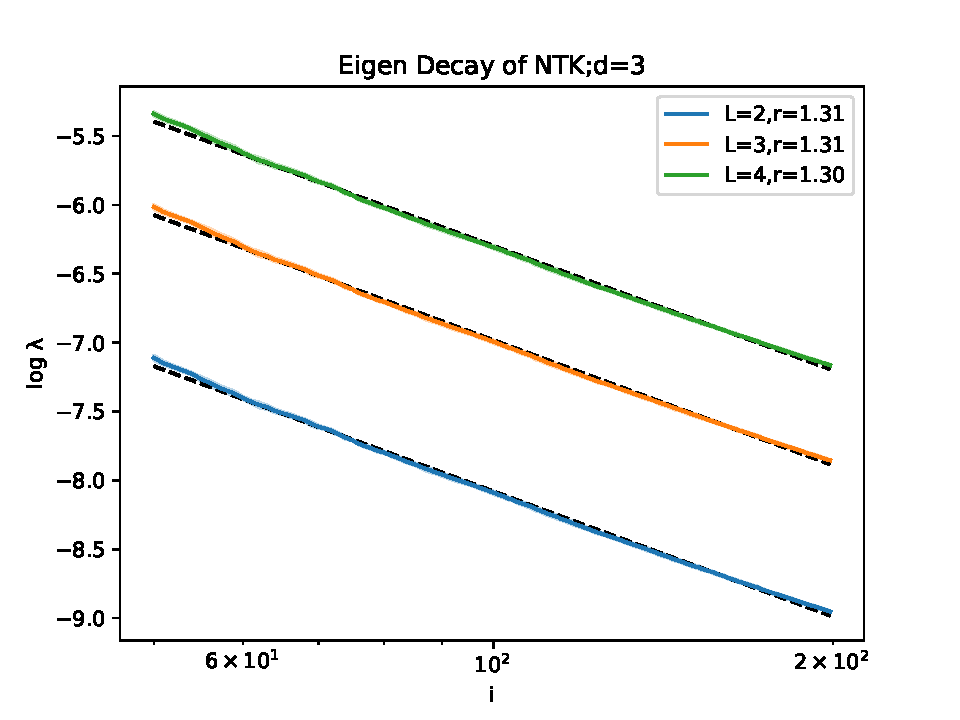
\includegraphics[width=1\linewidth]{fig/EigenNTKd3.pdf}
%     \end{minipage}%
%   }%
%   \subfigure{
%     \begin{minipage}[t]{0.5\linewidth}
%       \centering
%       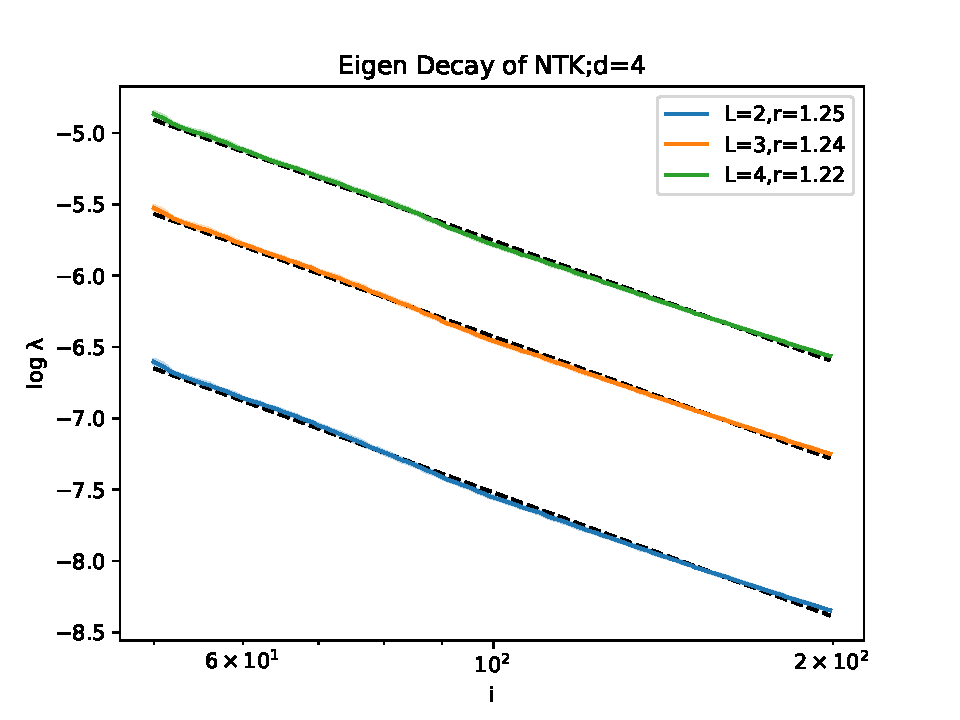
\includegraphics[width=1\linewidth]{fig/EigenNTKd4.pdf}
%     \end{minipage}%
%   }%

%   \subfigure{
%     \begin{minipage}[t]{0.5\linewidth}
%       \centering
%       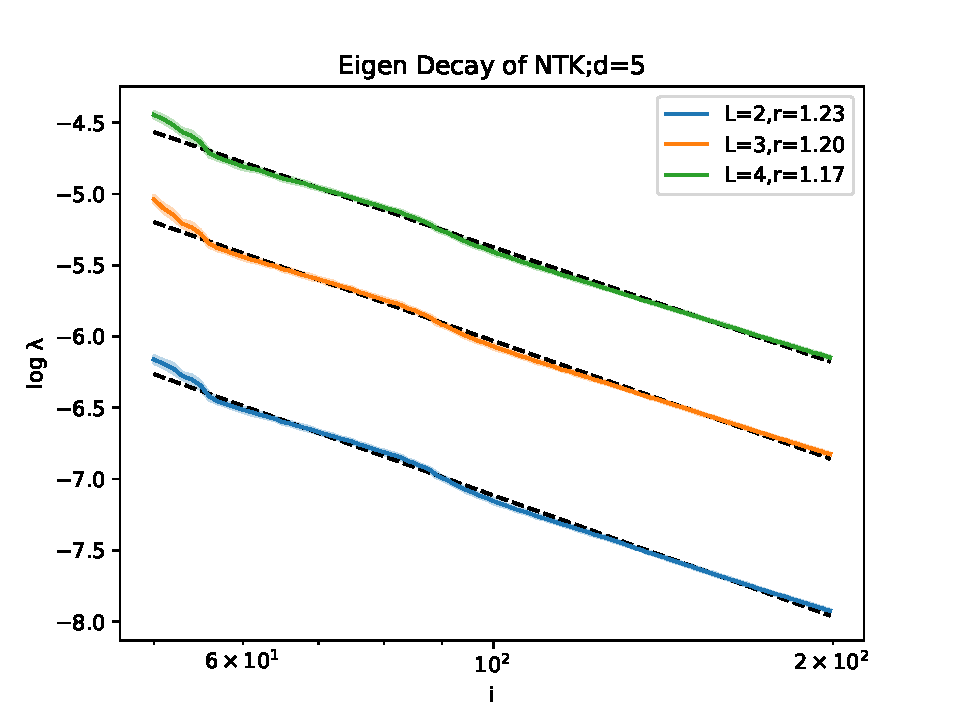
\includegraphics[width=1\linewidth]{fig/EigenNTKd5.pdf}
%     \end{minipage}%
%   }%
%   \subfigure{
%     \begin{minipage}[t]{0.5\linewidth}
%       \centering
%       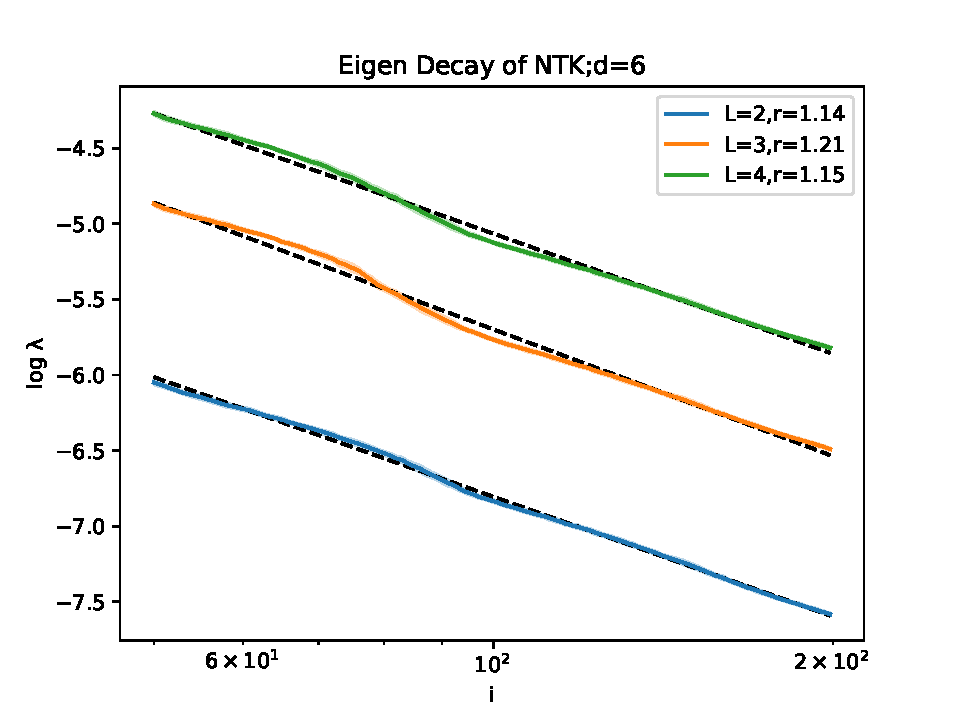
\includegraphics[width=1\linewidth]{fig/EigenNTKd6.pdf}
%     \end{minipage}%
%   }%


%   \centering
%   \caption{Eigenvalue decay of NTK under uniform distribution on $[-1,1]^d$,
%   where $i$ is selected in $[50,200]$ and $n = 1000$.
%   The dashed black line represents the log least-square fit and the decay rates $r$ are reported.}
%   \label{fig:EDR1}
%   \twocolumn
% \end{figure}


% \begin{table}[htb]
%   \centering
%   \begin{tabular}{c|ccc|ccc|ccc}
%     & \multicolumn{3}{c|}{$d=3$} & \multicolumn{3}{c|}{$d=4$} & \multicolumn{3}{c}{$d=5$} \\
%     \hline
%     Distribution & $L=2$ & $L=3$ & $L=4$ & $L=2$ & $L=3$ & $L=4$ & $L=2$ & $L=3$ & $L=4$ \\
%     \hline
%     $U(-1,1)$ & 1.31 & 1.31 & 1.30 & 1.25 & 1.24 & 1.22 & 1.23 & 1.20 & 1.17 \\
%     $U(0,1)$ & 1.33 & 1.33 & 1.32 & 1.26 & 1.26 & 1.25 & 1.14 & 1.13 & 1.12 \\
%     Triangular & 1.34 & 1.33 & 1.32 & 1.21 & 1.23 & 1.22 & 1.22 & 1.16 & 1.13 \\
%     Clipped normal & 1.28 & 1.30 & 1.28 & 1.26 & 1.24 & 1.21 & 1.11 & 1.09 & 1.06
%   \end{tabular}
%   \caption{Eigenvalue decay rates of NTK, where each entry of $\x$ is drawn independently from multiple distributions.
%   Triangular: $p(\x) = 1+x$, $x \in [-1,0]$, $p(\x) = 1-x$, $x \in [0,1]$;
%   Clipped normal: standard normal clipped into $(-10,10)$.}
%   \label{tab:1}
% \end{table}

% \cleardoublepage













